\lecture{CG(2); the beam equation and CG(3)}{Lectures 10--11 (combined)}{Math 6660 --- \texttt{missing.pdf} (colleague's notes)}

\noindent{\small\itshape These two lectures are missing from my own notebook;
the transcription below is from a classmate's notes, so the wording is his, not
mine. The material picks up mid-sentence from the adaptive criterion at the end
of Lecture 9.}

\begin{roadmap}[Lectures 10--11]
\roadq{Two questions: what if $O(h)$ is not good enough? And what changes when
the structure bends instead of stretches?}
\begin{roadlist}
\item \textbf{CG(2)}: add a midside node so each element carries a parabola.
  Rates improve to $O(h^{2})$ in energy and $O(h^{3})$ in $L^{2}$. The price is
  bandwidth --- the matrix stops being tridiagonal.
\item \textbf{The beam}, $u^{(iv)}=f$: four derivatives get shared two-and-two
  by integration by parts, so \emph{both} $u$ and $v$ now need two derivatives.
  The space jumps from $H^{1}$ to $H^{2}$.
\item That jump forbids kinks. Slope must match across element boundaries, so
  the elements must be \textbf{$C^{1}$} and each node carries a deflection
  \emph{and} a rotation.
\item \textbf{CG(3)}: cubic Hermite shape functions --- the classical beam
  element, derived from scratch.
\end{roadlist}
\payoff{Why a bar element has one dof per node and a beam element has two, and
why continuity requirements are a property of the \emph{equation}, not a
modelling choice.}
\end{roadmap}

% ##################################################################
\subsection*{Finishing the adaptive criterion}

\begin{equation}\label{eq:l10adapt}
  \text{If } E_{j}^{2}\le\frac{\eps^{2}}{c^{2}(M+1)}
  \text{ move to the next element; else refine.}
\end{equation}

% ##################################################################
\subsection*{CG(2) method}

Same problem as before,
\begin{equation}\label{eq:l10bvp}
  \left\{
  \begin{aligned}
    -(au')'&=f &&\text{on }(0,1),\\
    u(0)=u(1)&=0,
  \end{aligned}\right.
\end{equation}
with the same variational problem
\begin{equation}\label{eq:l10var}
  \int_0^1 a\,u'v'\dx=\int_0^1 f v\dx\qquad\forall\,v\in\Vsp ,
\end{equation}
\begin{equation}\label{eq:l10V}
  \Vsp=\Bigl\{v:\ \int_0^1\bigl(v^{2}+(v')^{2}\bigr)\dx<\infty,\ \
  v(0)=v(1)=0\Bigr\}.
\end{equation}
What changes is only the subspace. For CG(2),
\begin{equation}\label{eq:l10Vh}
  \Vh=\bigl\{v\in\Vsp:\ v|_{[x_{j-1},x_{j}]}=a_{j}+b_{j}x+c_{j}x^{2}\bigr\}.
\end{equation}

\medskip\noindent
\textbf{Key:} need to find a suitable basis for $\Vh$.

\medskip\noindent
\textbf{Mesh} $\Th$: $\;0=x_{0}<x_{1}<\dots<x_{M}<x_{M+1}=1$.

\medskip\noindent
The simplest way to write CG(2) is to use Lagrangian polynomials. To do this,
introduce a \emph{submesh}:

\begin{center}
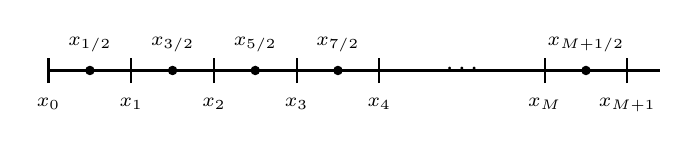
\begin{tikzpicture}[x=1.05cm,y=1cm]
  \draw[thick] (0,0) -- (7.4,0);
  \foreach \i/\lab in {0/{x_{0}},1/{x_{1}},2/{x_{2}},3/{x_{3}},4/{x_{4}}}{
     \draw[thick] (\i,-0.16) -- (\i,0.16);
     \node[below=2pt] at (\i,-0.16) {\scriptsize$\lab$};}
  \foreach \i/\lab in {6/{x_{M}},7/{x_{M+1}}}{
     \draw[thick] (\i,-0.16) -- (\i,0.16);
     \node[below=2pt] at (\i,-0.16) {\scriptsize$\lab$};}
  \foreach \i/\lab in {0.5/{x_{1/2}},1.5/{x_{3/2}},2.5/{x_{5/2}},3.5/{x_{7/2}},
                       6.5/{x_{M+1/2}}}{
     \filldraw (\i,0) circle (1.5pt);
     \node[above=3pt] at (\i,0) {\scriptsize$\lab$};}
  \node at (5,0.02) {$\cdots$};
\end{tikzpicture}
\end{center}

\noindent
The half-integer nodes need not be the midpoints, but we take them to be.

\begin{intuition}[what the extra node buys]
CG(1) fitted a straight line on each element, so two endpoint values pinned it
down. A parabola has three coefficients, so it needs a third condition, and the
cheapest place to put it is inside the element. The submesh node
$x_{j-1/2}$ is not a new mesh point --- the elements are unchanged --- it is
just a third \emph{degree of freedom} carried by the same element.
\end{intuition}

\begin{mechanics}
This is the three-node bar element. CG(1) is the 2-node linear bar with constant
strain; CG(2) is the 3-node quadratic bar whose strain varies linearly along the
element. The midside node is exactly the midside node of a Q8 or T6 element.
\end{mechanics}

% ------------------------------------------------------------------
\subsubsection*{The basis}

For a given element there are $3$ Lagrange polynomials:

\begin{center}
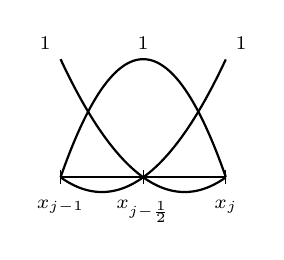
\begin{tikzpicture}[x=2.1cm,y=1.5cm]
  \draw[thick] (0,0) -- (1,0);
  \foreach \i/\lab in {0/{x_{j-1}},0.5/{x_{j-\frac12}},1/{x_{j}}}{
     \draw (\i,-0.06) -- (\i,0.06);
     \node[below=2pt] at (\i,-0.06) {\scriptsize$\lab$};}
  % L_left = 2t^2-3t+1 ; L_mid = 4t(1-t) ; L_right = 2t^2-t
  \draw[thick,domain=0:1,samples=60,smooth]
        plot (\x,{2*\x*\x-3*\x+1});
  \draw[thick,domain=0:1,samples=60,smooth]
        plot (\x,{4*\x*(1-\x)});
  \draw[thick,domain=0:1,samples=60,smooth]
        plot (\x,{2*\x*\x-\x});
  \node[above left]  at (0,1)   {\scriptsize$1$};
  \node[above]       at (0.5,1) {\scriptsize$1$};
  \node[above right] at (1,1)   {\scriptsize$1$};
\end{tikzpicture}
\end{center}

\noindent
As \emph{basis functions} over the whole mesh there are two shapes: the one
sitting at an integer node, which spans two elements, and the bubble sitting at
a half-integer node, which lives inside one element.

\begin{center}
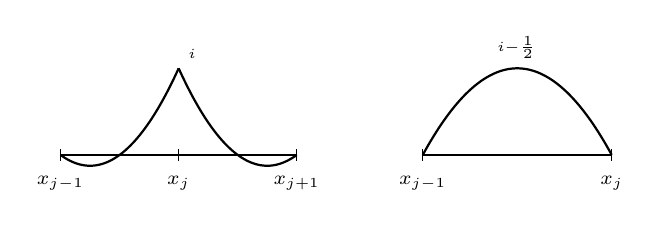
\begin{tikzpicture}[x=1.5cm,y=1.1cm]
  \begin{scope}
  \draw[thick] (0,0) -- (2,0);
  \foreach \i/\lab in {0/{x_{j-1}},1/{x_{j}},2/{x_{j+1}}}{
     \draw (\i,-0.07) -- (\i,0.07);
     \node[below=2pt] at (\i,-0.07) {\scriptsize$\lab$};}
  \draw[thick,domain=0:1,samples=50,smooth] plot (\x,{2*\x*\x-\x});
  \draw[thick,domain=1:2,samples=50,smooth]
        plot (\x,{2*(\x-1)*(\x-1)-3*(\x-1)+1});
  \node[above right] at (1,1) {\scriptsize$\phih_{i}$};
  \end{scope}
  \begin{scope}[xshift=4.6cm]
  \draw[thick] (0,0) -- (1.6,0);
  \foreach \i/\lab in {0/{x_{j-1}},1.6/{x_{j}}}{
     \draw (\i,-0.07) -- (\i,0.07);
     \node[below=2pt] at (\i,-0.07) {\scriptsize$\lab$};}
  \draw[thick,domain=0:1.6,samples=60,smooth]
        plot (\x,{4*(\x/1.6)*(1-\x/1.6)});
  \node[above] at (0.8,1) {\scriptsize$\phih_{i-\frac12}$};
  \end{scope}
\end{tikzpicture}
\end{center}

Explicitly,
\begin{equation}\label{eq:l10phii}
  \phih_{i}(x)=
  \begin{cases}
    \dfrac{2\bigl(x-x_{i+\frac12}\bigr)\bigl(x-x_{i+1}\bigr)}
          {\bigl(x_{i+1}-x_{i}\bigr)^{2}}, & x_{i}\le x\le x_{i+1},\\[2.2ex]
    \dfrac{2\bigl(x-x_{i-\frac12}\bigr)\bigl(x-x_{i-1}\bigr)}
          {\bigl(x_{i}-x_{i-1}\bigr)^{2}}, & x_{i-1}\le x\le x_{i},\\[2.2ex]
    0, & \text{otherwise,}
  \end{cases}
\end{equation}
\begin{equation}\label{eq:l10phihalf}
  \phih_{i-\frac12}(x)=
  \begin{cases}
    \dfrac{4\bigl(x_{i}-x\bigr)\bigl(x-x_{i-1}\bigr)}
          {\bigl(x_{i}-x_{i-1}\bigr)^{2}}, & x_{i-1}\le x\le x_{i},\\[2.2ex]
    0, & \text{otherwise.}
  \end{cases}
\end{equation}
Therefore
\begin{equation}\label{eq:l10span}
  \Vh=\operatorname{span}\bigl\{\phih_{\frac12},\phih_{1},\phih_{\frac32},
      \phih_{2},\dots,\phih_{M},\phih_{M+\frac12}\bigr\},
\end{equation}
so if $U\in\Vh$ then
\begin{equation}\label{eq:l10U}
  U(x)=\sum_{j=1}^{2M+1}\xi_{j}\,\phih_{j/2}(x).
\end{equation}

\medskip\noindent
\textbf{Note.} For any function $v\in\Vsp$,
\begin{equation}\label{eq:l10interp}
  \Pi_h v=\sum_{k=1}^{2M+1}v\bigl(x_{k/2}\bigr)\phih_{k/2}(x),
\end{equation}
and the test functions are $v=\phih_{i/2}(x)$ for $i=1,2,\dots,2M+1$.

% ------------------------------------------------------------------
\subsubsection*{CG(2) variational problem}

\begin{equation}\label{eq:l10cg2var}
  \sum_{j=1}^{2M+1}\xi_{j}\int_0^1 a(x)\,\phih'_{i/2}\phih'_{j/2}\dx
  =\int_0^1 f\,\phih_{i/2}\dx .
\end{equation}
This is a $(2M+1)\times(2M+1)$ symmetric positive definite system, \emph{but not
tridiagonal}.

\begin{pitfall}[the bandwidth changes, not just the size]
Going from CG(1) to CG(2) is not simply ``more unknowns.'' A basis function at
an integer node now overlaps the bubbles on \emph{both} neighbouring elements
and the integer node two slots away, so the matrix picks up a second
off-diagonal: it becomes pentadiagonal. Higher order buys accuracy per node and
pays for it in bandwidth --- the same trade a higher-order element makes in a
commercial solver.
\end{pitfall}

% ------------------------------------------------------------------
\subsubsection*{Example: $a\equiv1$ and $h_{j}=h$ for all $j$}

\noindent\textbf{Stiffness matrix.}

\medskip
\textcircled{\scriptsize1}\; $i=1,3,\dots,2M+1$ (the half-integer nodes):
\begin{align}
  A_{ii}&=\int_{x_{\frac{i}{2}-\frac12}}^{x_{\frac{i}{2}+\frac12}}
          \bigl(\phih'_{i/2}\bigr)^{2}\dx=\frac{16}{3h},
          \label{eq:l10Aodd}\\[0.4ex]
  A_{(i-1,i)}=A_{(i,i-1)}&=\int_{x_{\frac{i-1}{2}}}^{x_{\frac{i+1}{2}}}
          \phih'_{i/2}\,\phih'_{\frac{i-1}{2}}\dx=-\frac{8}{3h}.
          \label{eq:l10Aoddoff}
\end{align}

\textcircled{\scriptsize2}\; $i=2,4,6,\dots,2M$ (the integer nodes):
\begin{align}
  A_{ii}&=\int_{x_{\frac{i-1}{2}}}^{x_{\frac{i+1}{2}}}
          \bigl[\phih'_{i/2}\bigr]^{2}\dx=\frac{14}{3h},
          \label{eq:l10Aeven}\\[0.4ex]
  A_{(i,i-1)}=A_{(i-1,i)}&=\int_{x_{\frac{i-1}{2}}}^{x_{\frac{i}{2}}}
          \phih'_{i/2}\,\phih'_{\frac{i}{2}-\frac12}\dx=-\frac{8}{3h},
          \label{eq:l10Aevenoff1}\\[0.4ex]
  A_{(i,i-2)}=A_{(i-2,i)}&=\int_{x_{\frac{i-1}{2}}}^{x_{i/2}}
          \phih'_{i/2}\,\phih'_{\frac{i}{2}-1}\dx=\frac{1}{3h}.
          \label{eq:l10Aevenoff2}
\end{align}

\medskip\noindent\textbf{RHS vector.} Replace $f$ by its interpolant,
\begin{equation}\label{eq:l10fint}
  f\approx\widetilde{\Pi}_h f=\sum_{j=0}^{2M+2}f\bigl(x_{j/2}\bigr)\phih_{j/2}(x).
\end{equation}

\textcircled{\scriptsize1}\; $i=1,3,\dots,2M+1$:
\begin{equation}\label{eq:l10fodd}
  f_{i}=\sum_{j=1}^{2M+1}f\bigl(x_{j/2}\bigr)
        \int_{x_{\frac{i-1}{2}}}^{x_{\frac{i+1}{2}}}\phih_{j/2}\,\phih_{i/2}\dx
      =\frac{h}{15}\Bigl[f\bigl(x_{\frac{i-1}{2}}\bigr)
        +8f\bigl(x_{i/2}\bigr)+f\bigl(x_{\frac{i+1}{2}}\bigr)\Bigr].
\end{equation}

\textcircled{\scriptsize2}\; $i=2,4,\dots,2M$:
\begin{equation}\label{eq:l10feven}
  f_{i}=\frac{h}{30}\Bigl[-f\bigl(x_{\frac{i-2}{2}}\bigr)
        +2f\bigl(x_{\frac{i-1}{2}}\bigr)+8f\bigl(x_{i/2}\bigr)
        +2f\bigl(x_{\frac{i+1}{2}}\bigr)-f\bigl(x_{\frac{i+2}{2}}\bigr)\Bigr].
\end{equation}

\medskip\noindent
Therefore
\begin{equation}\label{eq:l10Amat}
  \bm{A}=\frac{1}{3h}
  \begin{bmatrix}
    16 & -8 &    &    &    &    &   \\
    -8 & 14 & -8 &  1 &    &    &   \\
       & -8 & 16 & -8 &    &    &   \\
       &  1 & -8 & 14 & -8 &  1 &   \\
       &    &    & \ddots & \ddots & \ddots & \\
       &    &    &  1 & -8 & 14 & -8\\
       &    &    &    &    & -8 & 16
  \end{bmatrix},
  \qquad \bm{A}\bm{x}=\bm{b}.
\end{equation}

\medskip\noindent
\textbf{Note (energy norm error).} Galerkin orthogonality gives
$\norm{u-U}_{E}\le\norm{u-v}_{E}$ for all $v\in\Vh$; taking $v=\Pi_h u$,
\begin{equation}\label{eq:l10eng}
  \boxed{\;\norm{u-U}_{E}\le c\,\norm{h^{2}u'''}\;}
\end{equation}

\noindent
\textbf{Note ($L^{2}$ error).}
\begin{equation}\label{eq:l10l2}
  \boxed{\;\norm{u-U}\le c\,\norm{h^{3}u'''}\;}
\end{equation}

\begin{intuition}[what the exponents say]
CG(1) gave $O(h)$ in energy and $O(h^{2})$ in $L^{2}$; CG(2) gives $O(h^{2})$
and $O(h^{3})$. Each extra polynomial degree buys one extra power of $h$ in both
norms, and the $L^{2}$ rate stays one power ahead of the energy rate --- the
duality argument of Lecture 8 is what produces that extra power, and it does not
care what degree the elements are.
\end{intuition}

% ##################################################################
\subsection*{Beam equation}

\begin{equation}\label{eq:l11beam}
  \left\{
  \begin{aligned}
    u^{(iv)}&=f &&\text{on }0<x<1,\\
    u(0)=u'(0)&=u(1)=u'(1)=0 .
  \end{aligned}\right.
\end{equation}

% ------------------------------------------------------------------
\subsubsection*{Variational problem}

Multiply by $v$ and integrate by parts twice:
\begin{align}
  \int_0^1 v\,u^{(iv)}\dx&=\int_0^1 f v\dx ,\label{eq:l11ibp0}\\
  -\int_0^1 v'u'''\dx+\underbrace{\bigl[v\,u'''\bigr]_0^1}_{=\,0}
     &=\int_0^1 f v\dx
     &&\text{(let } v(0)=v(1)=0),\label{eq:l11ibp1}\\
  \int_0^1 v''u''\dx-\underbrace{\bigl[v'u''\bigr]_0^1}_{=\,0}
     &=\int_0^1 f v\dx
     &&\text{(let } v'(0)=v'(1)=0),\label{eq:l11ibp2}
\end{align}
so
\begin{equation}\label{eq:l11weak}
  \int_0^1 u''v''\dx=\int_0^1 f v\dx .
\end{equation}
The space is
\begin{equation}\label{eq:l11V}
  \Vsp=\Bigl\{v:\ \int_0^1\bigl[v^{2}+(v')^{2}+(v'')^{2}\bigr]\dx<\infty,\ \
  v(0)=v(1)=v'(0)=v'(1)=0\Bigr\},
\end{equation}
and functions in $\Vsp$ are $C^{1}[0,1]$.

\medskip
\noindent\fbox{\parbox{0.93\linewidth}{%
\textbf{(Variational problem)} Find $u\in\Vsp$ such that
$\displaystyle\int_0^1 u''v''\dx=\int_0^1 f v\dx$ for all $v\in\Vsp$.}}

\begin{intuition}[why the space jumps from $H^{1}$ to $H^{2}$]
The bar equation lost one derivative to the test function and kept one, so
$\int(v')^{2}<\infty$ was enough. The beam equation has four derivatives to
share, two each, so now $\int(v'')^{2}<\infty$ is required. That extra
requirement is what forces $C^{1}$: a function with a corner has a jump in $v'$,
hence a delta in $v''$, hence $\int(v'')^{2}=\infty$. Kinks were legal for the
bar; they are illegal for the beam.
\end{intuition}

\begin{mechanics}
$\tfrac12\int(u'')^{2}$ is the bending strain energy $\tfrac12\int EI\,\kappa^{2}$
with $EI\equiv1$, since $u''$ is the curvature. Requiring finite bending energy
is requiring $u\in H^{2}$. And $C^{1}$ continuity is just the physical statement
that a beam does not develop a kink under a distributed load --- deflection
\emph{and} slope must match across an element boundary.
\end{mechanics}

% ------------------------------------------------------------------
\subsubsection*{Energy minimization}

Define
\begin{equation}\label{eq:l11F}
  F(w)=\frac12\int_0^1(w'')^{2}\dx-\int_0^1 f w\dx .
\end{equation}

\noindent\fbox{\parbox{0.93\linewidth}{%
\textbf{(Minimization problem)} Find $u\in\Vsp$ such that
$F(u)\le F(w)$ for all $w\in\Vsp$.}}

\medskip\noindent
\textbf{Claim.} (Var.\ Prob.)\;$\Longleftrightarrow$\;(Min.\ Prob.)

\medskip\noindent
($\Longrightarrow$) Assume $u\in\Vsp$ satisfies the variational problem. Let
$w=u+v\in\Vsp$. Then
\begin{align}
  F(w)=F(u+v)&=\underbrace{\frac12\int_0^1(u'')^{2}\dx-\int_0^1 fu\dx}_{=\,F(u)}
    \;+\;\frac12\int_0^1(v'')^{2}\dx
    \;+\;\underbrace{\int_0^1 u''v''\dx-\int_0^1 f v\dx}_{=\,0\ \text{by \eqref{eq:l11weak}}},
    \label{eq:l11expand}
\end{align}
so
\begin{equation}\label{eq:l11FwFu}
  F(w)=F(u)+\frac12\int_0^1(v'')^{2}\dx\;\ge\;F(u).
\end{equation}

\medskip\noindent
\textbf{Note.} $F(w)=F(u)\ \Rightarrow\ v''\equiv0\ \Rightarrow\ v\equiv0$
(due to the BCs) $\Rightarrow\ u\equiv w$.

\begin{intuition}[why $v''\equiv 0$ forces $v\equiv 0$ here]
$v''\equiv0$ only says $v$ is a straight line, $v=\alpha+\beta x$. It is the
four boundary conditions in \eqref{eq:l11V} that kill it: $v(0)=v'(0)=0$ already
force $\alpha=\beta=0$. For the bar, the same step used $v'\equiv0$ plus the two
Dirichlet conditions. Same mechanism, one derivative higher.
\end{intuition}

% ------------------------------------------------------------------
\subsection*{CG(3) method}

We need $\Vh\subseteq\Vsp$. On each element $[x_{j-1},x_{j}]$ we need a
polynomial that matches \emph{value and derivative} to its neighbours at
$x_{j-1}$ and $x_{j}$ --- that is $4$ conditions, so we need a cubic
($4$ coefficients):
\begin{equation}\label{eq:l11Vh}
  \Vh=\bigl\{v\in\Vsp:\ v|_{[x_{j-1},x_{j}]}
      =a_{j}+b_{j}x+c_{j}x^{2}+d_{j}x^{3}\bigr\}.
\end{equation}

\medskip\noindent
\textbf{Key:} find a basis for $\Vh$. Two basis functions are attached to each
node --- one controlling the value, one controlling the slope:

\begin{center}
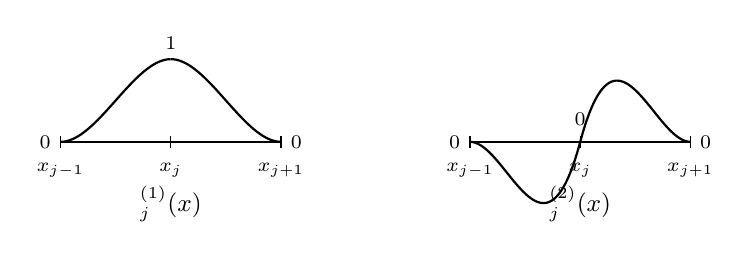
\begin{tikzpicture}[x=1.4cm,y=1.05cm]
  \begin{scope}
  \draw[thick] (0,0) -- (2,0);
  \foreach \i/\lab in {0/{x_{j-1}},1/{x_{j}},2/{x_{j+1}}}{
     \draw (\i,-0.07) -- (\i,0.07);
     \node[below=2pt] at (\i,-0.07) {\scriptsize$\lab$};}
  \draw[thick,domain=0:1,samples=60,smooth] plot (\x,{3*\x*\x-2*\x*\x*\x});
  \draw[thick,domain=1:2,samples=60,smooth]
        plot (\x,{3*(2-\x)*(2-\x)-2*(2-\x)*(2-\x)*(2-\x)});
  \node[above] at (1,1) {\scriptsize$1$};
  \node[left]  at (0,0) {\scriptsize$0$};
  \node[right] at (2,0) {\scriptsize$0$};
  \node at (1,-0.75) {\small$\phih_{j}^{(1)}(x)$};
  \end{scope}
  \begin{scope}[xshift=5.2cm]
  \draw[thick] (0,0) -- (2,0);
  \foreach \i/\lab in {0/{x_{j-1}},1/{x_{j}},2/{x_{j+1}}}{
     \draw (\i,-0.07) -- (\i,0.07);
     \node[below=2pt] at (\i,-0.07) {\scriptsize$\lab$};}
  % left: t^2(t-1) scaled ; right: u^2(1+u) with u=x-2
  \draw[thick,domain=0:1,samples=60,smooth]
        plot (\x,{5*(\x*\x*(\x-1))});
  \draw[thick,domain=1:2,samples=60,smooth]
        plot (\x,{5*((\x-2)*(\x-2)*(1+\x-2))});
  \node[left]  at (0,0) {\scriptsize$0$};
  \node[above] at (1,0.08) {\scriptsize$0$};
  \node[right] at (2,0) {\scriptsize$0$};
  \node at (1,-0.75) {\small$\phih_{j}^{(2)}(x)$};
  \end{scope}
\end{tikzpicture}
\end{center}

\noindent
They are fixed by the nodal table
\begin{center}\small
\renewcommand{\arraystretch}{1.35}
\begin{tabular}{@{}l|ccc@{}}
\toprule
 & $x_{j-1}$ & $x_{j}$ & $x_{j+1}$\\
\midrule
$\phih_{j}^{(1)}$      & $0$ & $1$ & $0$\\
$\bigl(\phih_{j}^{(1)}\bigr)'$ & $0$ & $0$ & $0$\\
$\phih_{j}^{(2)}$      & $0$ & $0$ & $0$\\
$\bigl(\phih_{j}^{(2)}\bigr)'$ & $0$ & $1$ & $0$\\
\bottomrule
\end{tabular}
\end{center}

\noindent
which gives
\begin{equation}\label{eq:l11phi1}
  \phih_{j}^{(1)}=
  \begin{cases}
    3\left(\dfrac{x-x_{j-1}}{x_{j}-x_{j-1}}\right)^{2}
      -2\left(\dfrac{x-x_{j-1}}{x_{j}-x_{j-1}}\right)^{3},
      & x_{j-1}\le x\le x_{j},\\[3ex]
    3\left(\dfrac{x-x_{j+1}}{x_{j}-x_{j+1}}\right)^{2}
      -2\left(\dfrac{x-x_{j+1}}{x_{j}-x_{j+1}}\right)^{3},
      & x_{j}\le x\le x_{j+1},\\[3ex]
    0, & \text{otherwise,}
  \end{cases}
\end{equation}
\begin{equation}\label{eq:l11phi2}
  \phih_{j}^{(2)}=
  \begin{cases}
    -\dfrac{1}{h_{j}}\bigl(x-x_{j-1}\bigr)^{2}
      +\dfrac{1}{h_{j}^{2}}\bigl(x-x_{j-1}\bigr)^{3},
      & x_{j-1}\le x\le x_{j},\\[3ex]
    \dfrac{1}{h_{j+1}}\bigl(x-x_{j+1}\bigr)^{2}
      +\dfrac{1}{h_{j+1}^{2}}\bigl(x-x_{j+1}\bigr)^{3},
      & x_{j}\le x\le x_{j+1},\\[3ex]
    0, & \text{otherwise.}
  \end{cases}
\end{equation}

\medskip\noindent\fbox{\parbox{0.93\linewidth}{%
\textbf{CG(3) FEM:} Find $U\in\Vh$ such that
$\displaystyle\int_0^1 U''v''\dx=\int_0^1 f v\dx$ for all $v\in\Vh$.}}

\begin{mechanics}
This is the Hermite beam element, exactly as it appears in a structural code.
$\phih_{j}^{(1)}$ and $\phih_{j}^{(2)}$ are the cubic Hermite shape functions
$N_{1},N_{2},N_{3},N_{4}$; node $j$ carries two degrees of freedom, a deflection
and a rotation. The table above is the statement $N_{i}(\text{dof}_{k})=
\delta_{ik}$ --- each shape function switches on one dof and leaves the other
three at zero. The $C^{1}$ requirement is why a beam element has a rotational
dof at all, while a bar element does not.
\end{mechanics}

\todoq{In the nodal table for the Hermite basis, the entry for
$\bigl(\phih_{j}^{(1)}\bigr)'$ at $x_{j}$ is written in a way that reads as a
$6$ in the scan. It has to be $0$ --- \eqref{eq:l11phi1} has a flat top at
$x_{j}$ --- and I have transcribed it as $0$. Worth a glance at the original.}

\todoq{Page~4 of the scan writes the two CG(2) error notes with $u'''$ on both
right-hand sides, $\norm{u-U}_{E}\le c\norm{h^{2}u'''}$ and
$\norm{u-U}\le c\norm{h^{3}u'''}$. Check whether the second was meant to carry
$u'''$ or $u^{(4)}$.}
